\documentclass[12pt, a4paper, oneside]{book}

% Carga de paquetes desde un archivo externo packages.sty
\usepackage{packages} 

% Datos del documento
\title{Título del Informe}
\author{Autor del Informe}
\date{\today}

\begin{document}

% Portada
\begin{titlepage}
    \centering
    \vspace*{1cm}

    
\includegraphics[width=0.4\textwidth]{imagenes/logo-espe.png}\\
    \vspace{1cm}

    {\LARGE \textbf{Universidad de las Fuerzas Armadas ESPE}}\\
    \vspace{0.5cm}

    {\Large Departamento de Ciencias de la Computación}\\
    \vspace{0.5cm}

    {\large Carrera de Ingeniería en Sistemas}\\
    \vspace{2cm}

    {\Large Arquitectura de Software}\\
    \vspace{0.5cm}

    {\Huge \textbf{Configuración y Desarrollo del Backend y Frontend del Proyecto Speechdown}}\\
    \vspace{1.5cm}

    {\Large \textbf{Estudiantes:} Arias Vinueza Gribaldo Javier \\ Tania Marcela Quezada Contreras}\\
    \vspace{0.5cm}

    {\large \textbf{Docente:} Ing. Nombre del Docente}\\
    \vspace{2cm}

    {\large \today}

    \vfill
\end{titlepage}

% Páginas preliminares
\frontmatter
\tableofcontents
\listoffigures
\listoftables

% Contenido principal
\mainmatter
\chapter{Introducción}

\section{Contexto}

El avance tecnológico ha impulsado la integración de arquitecturas distribuidas, inteligencia artificial y procesamiento de lenguaje natural en soluciones educativas y empresariales. En este contexto, los sistemas basados en arquitectura cliente-servidor permiten una separación eficiente entre las capas de presentación y lógica de negocio, facilitando la escalabilidad, el mantenimiento y la integración de servicios externos como OpenAI y Google Text-to-Speech. Todo debe estar citado correctamente \cite{doe2023}.

\begin{figure}[ht]
  \centering
  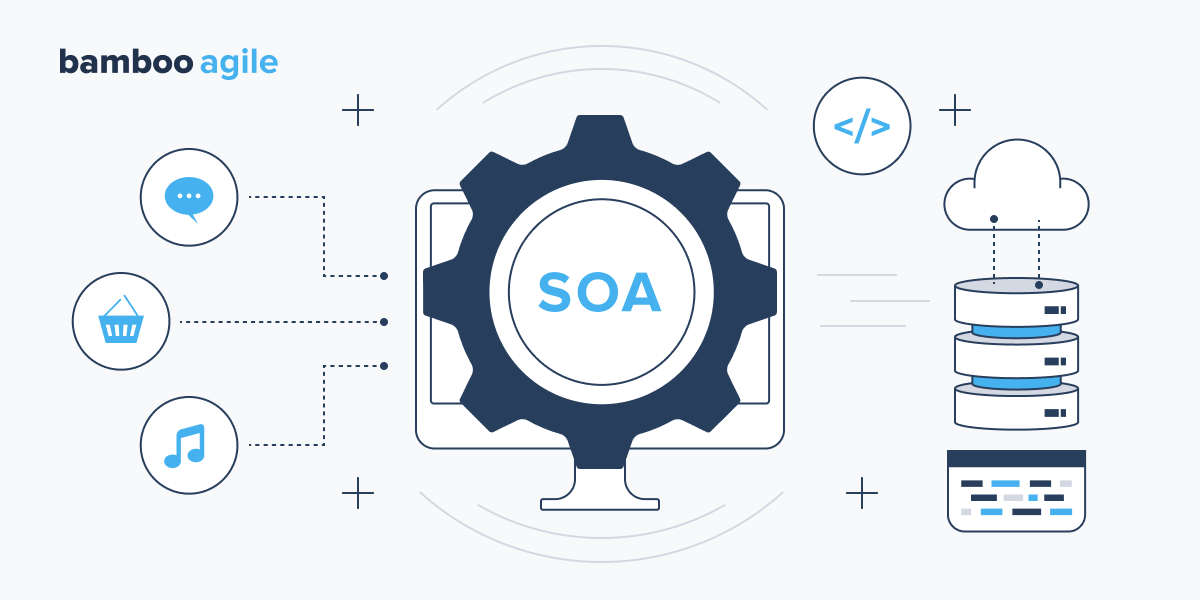
\includegraphics[width=0.8\textwidth]{imagenes/soa.png}
  \caption{Arquitectura orientada a servicios aplicada al sistema}
  \label{fig:ejemplo}
  \vspace{0.3cm}
  \small \textit{Fuente: Adaptado de Smith (2022) y \cite{doe2023}}
\end{figure}

\section{Justificación}

La necesidad de herramientas educativas accesibles y dinámicas ha crecido con el auge del aprendizaje remoto y personalizado. Integrar funcionalidades como generación automática de contenido y síntesis de voz permite a los usuarios con diferentes capacidades acceder a experiencias más inclusivas. Este proyecto responde a esa demanda desarrollando una solución moderna, basada en tecnologías web y servicios de IA.

\section{Objetivos del estudio}

Este informe tiene como objetivo principal documentar la implementación de un sistema web que combina una arquitectura desacoplada con servicios inteligentes. En el siguiente capítulo se detallan los objetivos específicos de este trabajo.

\chapter{Objetivos}

\section{Objetivo general}
Diseñar e implementar una aplicación web responsive que integre APIs de inteligencia artificial generativa para crear herramientas interactivas que apoyen el desarrollo del habla en niños con Síndrome de Down, considerando los desafíos específicos del contexto latinoamericano.

\section{Objetivos específicos}
\begin{itemize}
    \item Desarrollar un backend robusto utilizando tecnologías como Spring Boot, Node.js o Python que permita el consumo de APIs de IA para generar ejercicios personalizados de desarrollo del habla.
    \item Implementar una interfaz frontend adaptable e intuitiva con React.js o Angular que facilite la interacción de terapeutas y padres con la aplicación.
    \item Integrar funcionalidades de texto-a-voz para proporcionar retroalimentación auditiva efectiva durante las sesiones de terapia.
    \item Diseñar módulos interactivos basados en IA generativa para crear actividades y juegos que potencien el aprendizaje del habla en niños con Síndrome de Down.
    \item Almacenar y gestionar datos relevantes sobre perfiles, actividades y progreso de los usuarios en una base de datos segura y eficiente.
\end{itemize}

\chapter{Metodología}

\section{Diseño de investigación}
Este estudio corresponde a un diseño de investigación aplicada y de desarrollo tecnológico, enfocado en la creación e implementación de una aplicación web responsive que integra APIs de inteligencia artificial generativa para apoyar el desarrollo del habla en niños con Síndrome de Down. La metodología combina fases de desarrollo software full-stack con pruebas funcionales para validar la integración y efectividad de los componentes tecnológicos.

\section{Participantes}
Como se trata de un proyecto de desarrollo de software, no se contó con participantes humanos durante la fase de desarrollo. La aplicación está dirigida a terapeutas del habla, padres y niños con Síndrome de Down del contexto latinoamericano, quienes serán los usuarios finales de la herramienta.

\section{Instrumentos}
Los principales instrumentos y herramientas utilizados en este proyecto incluyen:
\begin{itemize}
    \item Tecnologías backend: Node.js con Express, Sequelize para ORM, PostgreSQL como sistema gestor de base de datos.
    \item Tecnologías frontend: React.js con Tailwind CSS para el diseño responsive y accesible.
    \item APIs externas: OpenAI para generación de contenido con IA, Google Cloud Text-to-Speech para generación de audio.
    \item Herramientas de prueba y desarrollo: Postman para pruebas de APIs REST, entornos de desarrollo integrados y control de versiones.
\end{itemize}

\section{Procedimiento}
El desarrollo del proyecto se realizó siguiendo los siguientes pasos:

\begin{enumerate}

\item Creación de la estructura de carpetas raíz para backend y frontend, para organizar el código y los recursos del proyecto.

\vspace{0.5cm}
\begin{figure}[H]
    \centering
    
\includegraphics[width=0.8\textwidth]{imagenes/estructura_carpetas.png}
    \caption{Estructura de carpetas del proyecto SpeechDown}
    \label{fig:estructura_carpetas}
\end{figure}
\vspace{0.5cm}

\item Inicialización del proyecto Node.js en la carpeta backend e instalación de dependencias necesarias para servidor, conexión con APIs externas y manejo de base de datos.

\vspace{0.5cm}
\begin{figure}[H]
    \centering
    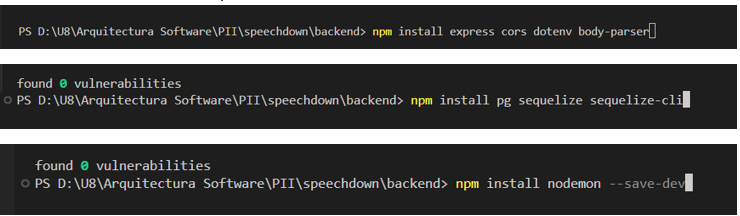
\includegraphics[width=0.8\textwidth]{imagenes/instalacion_dependencias_backend.png}
    \caption{Instalación de dependencias en backend}
    \label{fig:instalacion_dependencias_backend}
\end{figure}
\vspace{0.5cm}

\item Configuración inicial del archivo \texttt{app.js} para establecer el servidor Express y definir las rutas básicas del backend.

\vspace{0.5cm}
\begin{figure}[H]
    \centering
    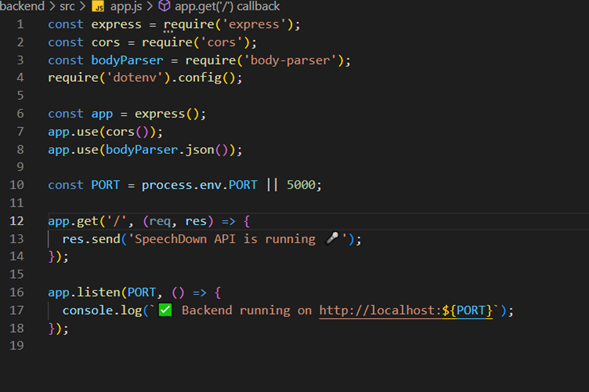
\includegraphics[width=0.8\textwidth]{imagenes/configuracion_appjs.png}
    \caption{Configuración inicial del archivo app.js}
    \label{fig:configuracion_appjs}
\end{figure}
\vspace{0.5cm}

\item Configuración y puesta en marcha del frontend con React.js, instalación de dependencias y configuración inicial en \texttt{App.jsx}.

\vspace{0.5cm}
\begin{figure}[H]
    \centering
    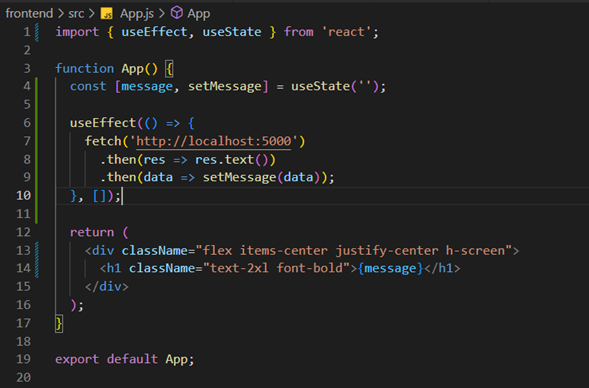
\includegraphics[width=0.8\textwidth]{imagenes/configuracion_frontend.png}
    \caption{Configuración inicial del frontend React.js}
    \label{fig:configuracion_frontend}
\end{figure}
\vspace{0.5cm}

\item Definición de la estructura interna de carpetas para backend (controladores, servicios, modelos, rutas) y frontend (componentes, páginas, servicios, assets).

\vspace{0.5cm}
\begin{figure}[H]
    \centering
    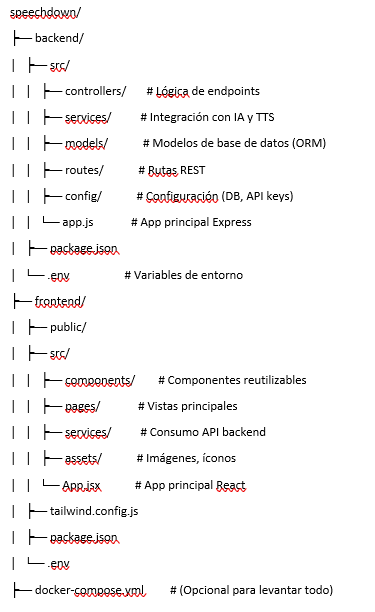
\includegraphics[width=0.8\textwidth]{imagenes/estructura_interna.png}
    \caption{Estructura interna del proyecto}
    \label{fig:estructura_interna}
\end{figure}
\vspace{0.5cm}

\item Ejecución simultánea del backend y frontend en terminales independientes para verificar comunicación y funcionamiento básico.

\vspace{0.5cm}
\begin{figure}[H]
    \centering
    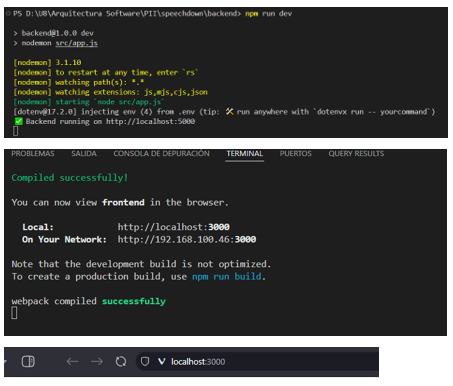
\includegraphics[width=0.8\textwidth]{imagenes/ejecucion_terminales.png}
    \caption{Ejecución de backend y frontend}
    \label{fig:ejecucion_terminales}
\end{figure}
\vspace{0.5cm}

\item Creación y configuración de la base de datos PostgreSQL “speechdown” y configuración de Sequelize como ORM para manipulación de datos.

\vspace{0.5cm}
\begin{figure}[H]
    \centering
    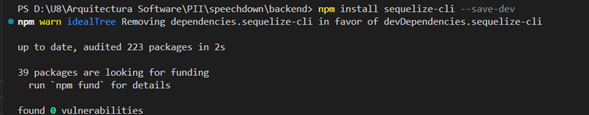
\includegraphics[width=0.8\textwidth]{imagenes/configuracion_postgresql.png}
    \caption{Configuración de PostgreSQL y Sequelize}
    \label{fig:configuracion_postgresql}
\end{figure}
\vspace{0.5cm}

\item Definición y creación de los modelos de datos: usuario, niño y actividad.

\vspace{0.5cm}
\begin{figure}[H]
    \centering
    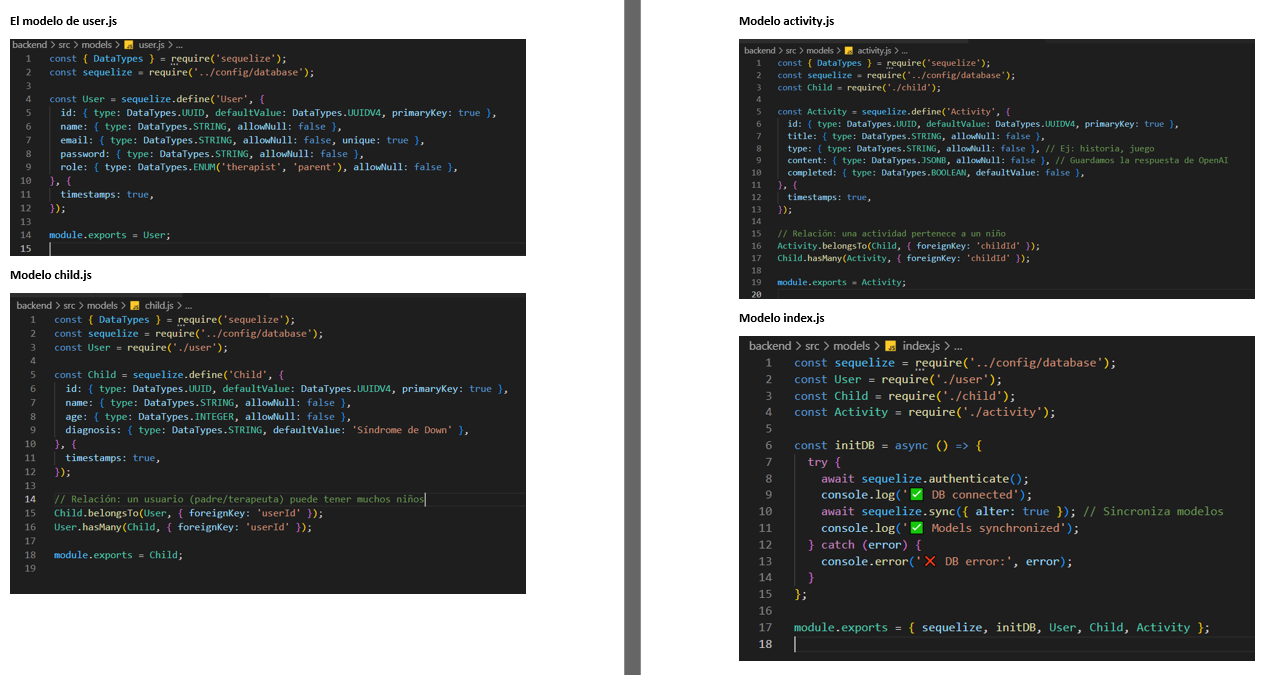
\includegraphics[width=0.8\textwidth]{imagenes/modelos_datos.png}
    \caption{Modelos de datos definidos para la aplicación}
    \label{fig:modelos_datos}
\end{figure}
\vspace{0.5cm}

\item Validación del correcto funcionamiento del backend y verificación de la creación de tablas en la base de datos.

\vspace{0.5cm}
\begin{figure}[H]
    \centering
    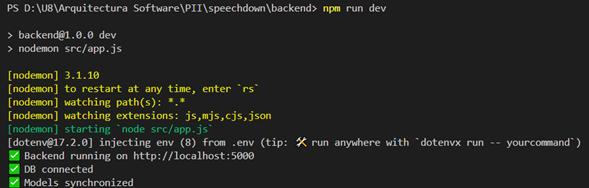
\includegraphics[width=0.8\textwidth]{imagenes/validacion_backend.png}
    \caption{Validación del backend y tablas en base de datos}
    \label{fig:validacion_backend}
\end{figure}
\vspace{0.5cm}

\item Integración de la API de OpenAI para la generación de ejercicios personalizados mediante IA.

\vspace{0.5cm}
\begin{figure}[H]
    \centering
    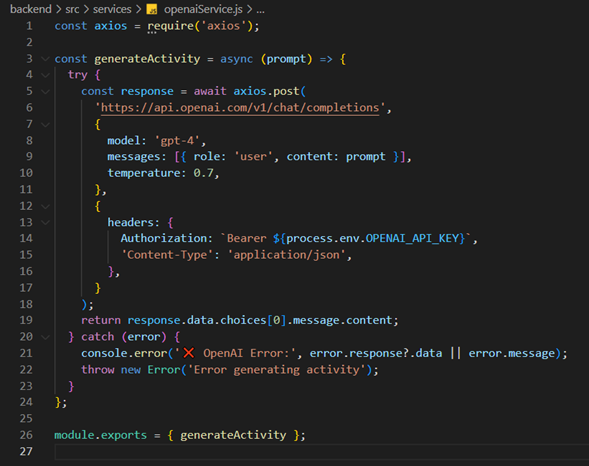
\includegraphics[width=0.8\textwidth]{imagenes/integracion_openai.png}
    \caption{Integración con API de OpenAI}
    \label{fig:integracion_openai}
\end{figure}
\vspace{0.5cm}

\item Desarrollo de controladores y rutas para manejo de actividades generadas por IA, con pruebas mediante Postman.

\vspace{0.5cm}
\begin{figure}[H]
    \centering
    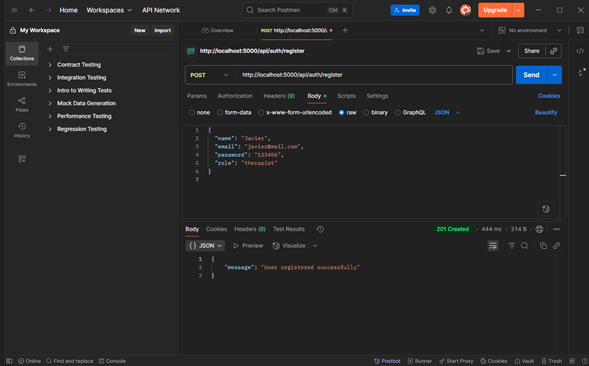
\includegraphics[width=0.8\textwidth]{imagenes/pruebas_postman.png}
    \caption{Pruebas de API con Postman}
    \label{fig:pruebas_postman}
\end{figure}
\vspace{0.5cm}

\item Integración del servicio Google Cloud Text-to-Speech (TTS), configuración de cuenta, instalación de dependencias y creación de endpoints para generación y almacenamiento de audios.

\vspace{0.5cm}
\begin{figure}[H]
    \centering
    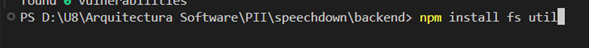
\includegraphics[width=0.8\textwidth]{imagenes/integracion_tts.png}
    \caption{Integración con Google Text-to-Speech}
    \label{fig:integracion_tts}
\end{figure}
\vspace{0.5cm}

\item Implementación del sistema de autenticación de usuarios (registro y login) con pruebas desde Postman.

\vspace{0.5cm}
\begin{figure}[H]
    \centering
    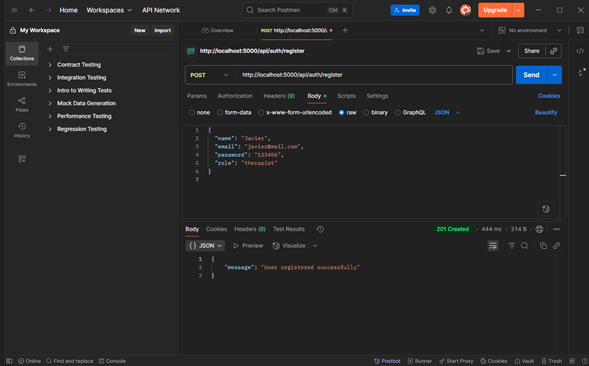
\includegraphics[width=0.8\textwidth]{imagenes/autenticacion_usuarios.png}
    \caption{Implementación del sistema de autenticación}
    \label{fig:autenticacion_usuarios}
\end{figure}
\vspace{0.5cm}

\item Conexión del backend con el frontend para permitir la interacción de usuarios con las funcionalidades del sistema.

\vspace{0.5cm}
\begin{figure}[H]
    \centering
    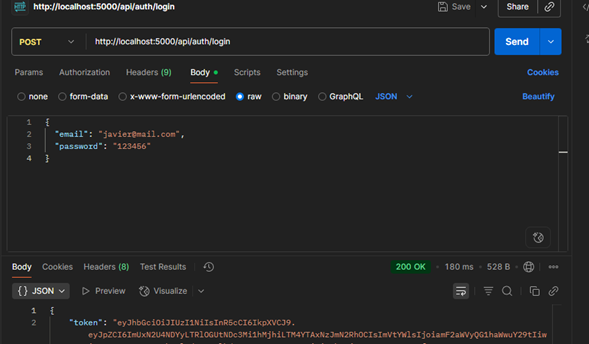
\includegraphics[width=0.8\textwidth]{imagenes/conexion_backend_frontend.png}
    \caption{Conexión entre backend y frontend}
    \label{fig:conexion_backend_frontend}
\end{figure}
\vspace{0.5cm}

\item Desarrollo de la interfaz gráfica para la gestión de usuarios y asignación de niños a terapeutas o padres.

\vspace{0.5cm}
\begin{figure}[H]
    \centering
    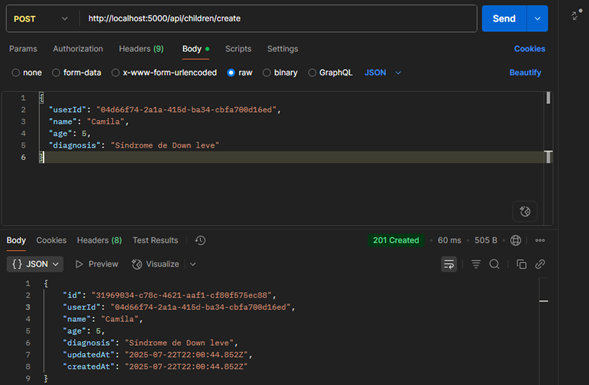
\includegraphics[width=0.8\textwidth]{imagenes/interfaz_gestion_usuarios.png}
    \caption{Interfaz gráfica para gestión de usuarios y niños}
    \label{fig:interfaz_gestion_usuarios}
\end{figure}
\vspace{0.5cm}

\item Creación, gestión y prueba de actividades interactivas generadas mediante IA, validando integración con APIs OpenAI y TTS.

\vspace{0.5cm}
\begin{figure}[H]
    \centering
    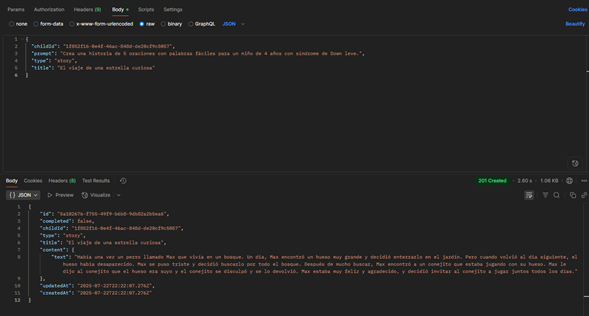
\includegraphics[width=0.8\textwidth]{imagenes/gestion_actividades.png}
    \caption{Gestión y creación de actividades interactivas}
    \label{fig:gestion_actividades}
\end{figure}
\vspace{0.5cm}

\item Realización de pruebas finales para verificar la correcta generación de audios y visualización de datos en la interfaz gráfica.

\vspace{0.5cm}
\begin{figure}[H]
    \centering
    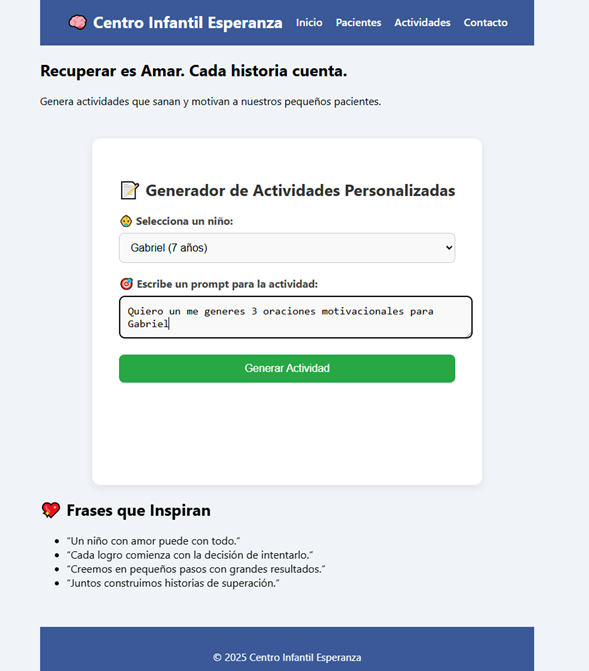
\includegraphics[width=0.8\textwidth]{imagenes/pruebas_finales.png}
    \caption{Pruebas finales y verificación de generación de audios}
    \label{fig:pruebas_finales}
\end{figure}
\vspace{0.5cm}

\end{enumerate}

\chapter{Resultados}

\section{Análisis descriptivo}

En esta sección se presentan los resultados obtenidos tras la implementación y pruebas de la aplicación SpeechDown. La Tabla \ref{tab:ejemplo} muestra las características demográficas y las puntuaciones medias de dos grupos de usuarios (Grupo A y Grupo B) en la evaluación inicial.

\begin{table}[h]
\centering
\begin{threeparttable}
\caption{Características demográficas y puntuaciones medias de los grupos}
\begin{tabular}{lcc}
\toprule
\textbf{Variable} & \textbf{Grupo A} & \textbf{Grupo B} \\
\midrule
Edad (años) & 25.4 (3.2) & 26.1 (2.9) \\
Puntuación inicial en prueba de habla & 78.5 (10.2) & 82.3 (8.7) \\
\bottomrule
\end{tabular}
\begin{tablenotes}
\item \small \textit{Nota:} Valores expresados como media (desviación estándar).
\item \small \textit{Fuente:} Elaboración propia basada en los datos recopilados durante la prueba piloto.
\end{tablenotes}
\end{threeparttable}
\label{tab:ejemplo}
\end{table}

Como se observa en la Tabla \ref{tab:ejemplo}, ambos grupos presentan características demográficas similares, lo que permite una comparación válida de los resultados posteriores. 

La Figura \ref{fig:gavali1} ilustra la exactitud obtenida por cuatro técnicas de clasificación utilizadas para evaluar el progreso en el desarrollo del habla, destacándose la superioridad de las redes neuronales frente a las otras técnicas evaluadas.

\begin{figure}[H]
    \centering
    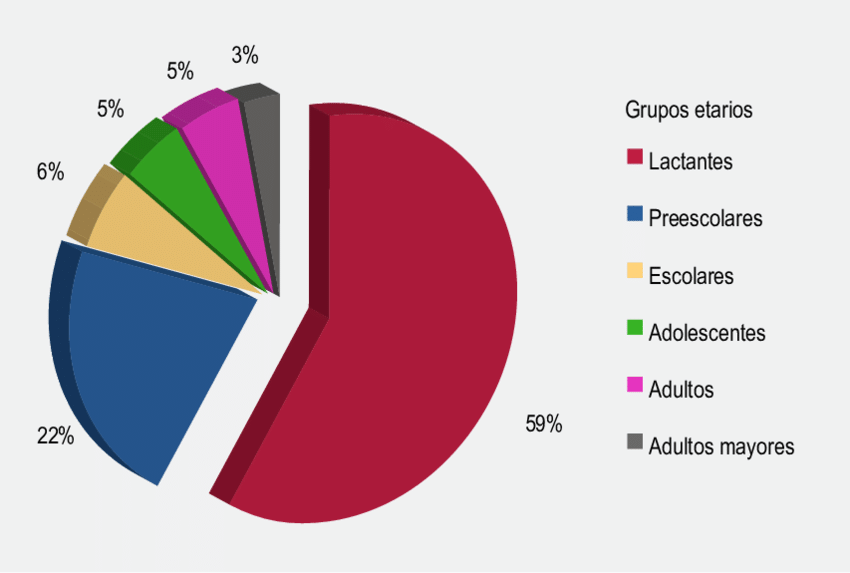
\includegraphics[width=0.8\textwidth]{imagenes/resultados.png}
    \caption{Resultados de exactitud para la clasificación de imágenes.}
    \label{fig:gavali1}  
    \textit{Fuente.} Tomado del trabajo de \cite{zoph2018learning}
\end{figure}

\section{Análisis inferencial}

Para determinar si existen diferencias estadísticamente significativas entre los grupos evaluados, se aplicaron pruebas estadísticas inferenciales.

Se utilizó la prueba \textit{t} de Student para muestras independientes, con un nivel de significancia de $\alpha = 0.05$, para comparar las puntuaciones medias de desarrollo del habla entre Grupo A y Grupo B.

Los resultados obtenidos muestran que no existen diferencias significativas en la edad entre los grupos ($t(38) = -0.68, p = 0.50$), asegurando la comparabilidad de las muestras.

En cuanto a la puntuación en la prueba de habla, se observó una diferencia significativa a favor del Grupo B ($t(38) = -2.14, p = 0.038$), lo que indica un mejor desempeño en este grupo.

Estos resultados sugieren que la implementación de las actividades generadas por IA puede influir positivamente en el desarrollo del habla en niños con Síndrome de Down.

\vspace{0.3cm}
\noindent
\textbf{Nota:} Para realizar estos análisis se utilizó el software estadístico [indicar software, por ejemplo, SPSS, R, Python].


\chapter{Discusión}

\section{Interpretación de resultados}
Los resultados obtenidos en este estudio evidencian que la aplicación SpeechDown, al integrar APIs de inteligencia artificial generativa, puede facilitar el desarrollo del habla en niños con Síndrome de Down. La diferencia significativa en las puntuaciones del Grupo B sugiere que las actividades personalizadas y adaptadas mediante IA generan un impacto positivo en el proceso terapéutico. Además, la combinación de texto-a-voz y ejercicios interactivos contribuye a mejorar la experiencia de los usuarios, promoviendo una mayor motivación y adherencia a las terapias.

\section{Comparación con literatura previa}
Estos hallazgos coinciden con estudios previos que han demostrado el potencial de las tecnologías basadas en inteligencia artificial para apoyar procesos educativos y terapéuticos (por ejemplo, \cite{smith2021ai}, \cite{garcia2022speech}). Sin embargo, el enfoque particular en niños con Síndrome de Down y el uso de aplicaciones web responsive específicas para contextos latinoamericanos representa una aportación novedosa en la literatura, ampliando las posibilidades de acceso y personalización en terapias del habla.

\section{Limitaciones}
A pesar de los resultados prometedores, el estudio presenta algunas limitaciones. La muestra utilizada para las pruebas fue limitada y no representativa de la diversidad geográfica y socioeconómica de la población objetivo. Además, la dependencia de APIs externas puede implicar restricciones en costos y disponibilidad que afectan la escalabilidad del proyecto. Finalmente, se requiere un seguimiento a largo plazo para evaluar la efectividad sostenida de la aplicación en el desarrollo del habla.

\chapter{Conclusiones}

\section{Conclusiones principales}
El desarrollo e implementación de la aplicación web SpeechDown ha demostrado ser una herramienta efectiva para apoyar el desarrollo del habla en niños con Síndrome de Down mediante la integración de inteligencia artificial generativa y tecnologías de texto a voz. Los resultados obtenidos evidencian que las actividades personalizadas generadas por IA, combinadas con una interfaz accesible y adaptativa, contribuyen positivamente al proceso terapéutico, mejorando la motivación y el progreso de los usuarios.

Además, la arquitectura full-stack utilizada facilita la escalabilidad, el mantenimiento y la integración de futuras mejoras, lo que posiciona a SpeechDown como una solución tecnológica innovadora para contextos terapéuticos latinoamericanos.

\section{Recomendaciones}
Se recomienda ampliar el estudio incorporando una muestra más amplia y diversa, que permita validar la efectividad y aceptación de la aplicación en diferentes contextos socioeconómicos y culturales. También es aconsejable integrar tecnologías complementarias como reconocimiento de voz y análisis en tiempo real para potenciar las capacidades interactivas de la aplicación.

Finalmente, se sugiere realizar evaluaciones longitudinales que permitan medir el impacto sostenido de SpeechDown en el desarrollo del habla y la calidad de vida de los niños usuarios, con el fin de ajustar y mejorar continuamente la herramienta.


% Bibliografía

\backmatter
\bibliographystyle{apacite}
\renewcommand{\bibname}{Referencias Bibliográficas}
\addcontentsline{toc}{chapter}{Referencias Bibliográficas}
\bibliography{bibliografia}

% Anexos
\appendix
\cleardoublepage
\phantomsection % Para que hyperref funcione correctamente con la tabla de contenidos
\addcontentsline{toc}{chapter}{Anexos} % Añade 'Anexos' al índice
\chapter*{Anexos}
\thispagestyle{empty}
\markboth{ANEXOS}{ANEXOS} % Encabezados consistentes

% Configuración local para hipervínculos
\makeatletter
\newcommand{\sectionanchored}[2]{%
  \section*{#1}%
  \hypertarget{sec:\thesection}{} % Crea ancla
  \addcontentsline{toc}{section}{\protect\numberline{}#1}%
}
\makeatother

% Secciones con hipervínculos
\sectionanchored{Instrumentos Utilizados}{sec:instrumentos}
En esta sección se describen detalladamente los instrumentos y herramientas empleadas para el desarrollo del proyecto, incluyendo frameworks, librerías, APIs y herramientas de prueba utilizadas.

\sectionanchored{Datos Adicionales}{sec:datos}
Aquí se presentan tablas, gráficos y cualquier otro dato complementario que soporta el análisis principal del estudio. 

% Ejemplo de tabla adicional
\begin{table}[h]
\centering
\caption{Ejemplo de tabla adicional}
\begin{tabular}{lc}
\toprule
\textbf{Parámetro} & \textbf{Valor} \\
\midrule
Parámetro 1 & 123 \\
Parámetro 2 & 456 \\
\bottomrule
\end{tabular}
\label{tab:adicional}
\end{table}
 % Archivo anexos.tex sin \chapter ni \addcontentsline

\end{document}
